\chapter{Evaluation}\label{chap:evaluation}
This chapter describes the tests and experiments we setup in order to evaluate our solution. 
We setup \num{4} tests, one in each of the following sections. 
The first test, described in \Cref{sec:gestureperformance}, we perform, 
is to measure the performance of the gesture recognizer described in \Cref{sec:gesturerecognition}. 
Then we evaluate the correctness of the gesture recognizer in \Cref{sec:gesturecorrectness}.
To test the precision of our indoor location, 
we perform precision tests on the Estimote SDK in \Cref{sec:estimoteprecision}.
Being able to detect points, and thus when to start recognizing gestures, we implemented a point detector. This detector is evaluated in \Cref{sec:evaluation:pointing}.
The server and the smart hub, HomePort, is briefly evaluated in \Cref{sec:servereval}.
Finally we test the system as a whole in \Cref{sec:evaluation:system-correctness}.

\section{Performance of Gesture Recognition}\label{sec:gestureperformance}
Gesture recognition is a core part of our solution and it is being performed often. 
Since the gesture recognition is being performed by a device with somewhat low performance,
it is important that the gesture recognition is not computationally heavy.
In \Cref{sec:requirements-specification} we set a requirement of less than \SI{200}{\milli\second} for each gesture recognition.
We test the performance by gradually populating the database with gesture traces, 
and see how fast we can recognize a random gesture input.
We expect the number of gesture traces in the database to increase the recognition time.

For this setup, we add five gesture traces at a time. 
This is to simulate training a gesture five times, 
as recommended by the \$3 Gesture Recognition paper \cite{threedollar}. 
We then generate a random gesture input, 
and run the recognition function on it ten times, 
logging the execution time.
We repeat this until there is a total of \num{100} gesture traces in the database, 
which corresponds to \num{20} unique gestures.

We performed this test six times on an iPhone 5, 
with a \SI{1.3}{\giga\hertz} dual-core ARM processor and \SI{1}{\giga\byte} RAM, running iOS 9.1.
This device is more powerful than most wearables, 
but newer wearables such as the Samsung Gear S2 has a \SI{1}{\giga\hertz} dual core CPU with \SI{512}{\mega\byte} RAM, 
so the results from this section are comparable with newer and upcoming wearable devices.

\begin{figure}[!htb]
    \centering
    \begin{tikzpicture}
  \begin{axis}[ybar,bar width=2pt]
    \addplot table[x=gestureNo, y=time] {data/three-dollar-test-results/results/10xrecognize/2015-11-25 12.36.29.csv};   
  \end{axis}
\end{tikzpicture}
    \caption{Graph showing the time of recognizing gestures, with increasing number of gesture traces. Each unique gesture is training \num{5} times.}
    \label{fig:performancegraph}
\end{figure}

During testing we noticed that the ``Three Dollar Gesture Recognizer'' used a high amount of memory. 
Furthermore it did not properly release this memory, 
and as a result the application would terminate during tests, 
if we ran them for too long.
\Cref{fig:threedollarmemory} shows the amount of memory, 
used by our application, 
in a timespan of one minute and thirteen seconds, 
starting at the point where the application was launched on the iPhone. 
The first dotted line shows the time when the test began, 
and the second dotted line shows when the test finished, 
and where the \$3 Gesture Recognizer started cleaning up its resources.
However, as the graph shows, the memory use stays high after cleanup. %Thalley: Kunne det ikke blot være pga. iOS's måde at håndtere memory på? 
This issue is the reason we only repeat recognition ten times for each gesture, 
as more would cause the application to shut down due to excessive memory usage. %Thalley: Kan vi se hvor mange gestures den højst kan recognize før det er et problem? 

\begin{figure}[!htb]
  \begin{tikzpicture}
    \centering
    \node[anchor=south west,inner sep=0] (image) at (0,0) {\includegraphics[width=0.7\textwidth]{images/three-dollar-memory-use.png}};
    \begin{scope}[x={(image.south east)},y={(image.north west)}]
    \draw[red,ultra thick, dotted] (0.45,0.08) -- (0.45,0.97);
    \draw[red,ultra thick, dotted] (0.73,0.08) -- (0.73,0.97);
    \end{scope}
  \end{tikzpicture}
  \caption{RAM usage of the \$3 Gesture Recognizer. The first dashed line shows when it starts recognizing, and the second dashed line shows when it stops. The area after the second dashed line shows that it does \emph{not} clean up the memory after use.}
  \label{fig:threedollarmemory}
\end{figure}

\subsection{Performance of Gesture Recognition Conclusion}
The result from \Cref{fig:performancegraph} shows that the time spent recognizing a gesture 
increases linearly with the amount of gesture traces in the database.
The computational time is well below the requirement of \SI{200}{\milli\second},
thus the performance of the \$3 Gesture Recognizer is adequate for our system. 
The memory issues encountered during testing, however, 
showed that it might not be an appropriate solution, 
if the system is to run for a prolonged period of time.
With a proper implementation of the \$3 Gesture Recognizer, 
this can be avoided. 

\subsubsection{Considerations}
While the computational time is low, 
the memory used, as seen by \Cref{fig:threedollarmemory}, is high (up to \SI{405.1}{\mega\byte}). 
For the iPhone that we tested on, this is an issue as the operating system terminates the application due to high memory pressure. With less memory available which may be the case on smaller wearables, this would be an even more critical issue.

Furthermore, we tested by generating random gestures programmatically. 
We assume that the \$3 Gesture Recognizer spend the same amount of time on each gesture, 
regardless of whether it exists in the gesture database or if it is a completely random trace. 


\section{Correctness Rate of Gesture Recognition}\label{sec:gesturecorrectness}
%Thalley: if this changes, make sure to change this section
%Thalley: If we want to perform our own tests based on e.g. the gestures in previous section, rewrite this
We are using the \$3 Gesture Recognizer and they have in their paper, 
presenting the recognition system, performed this test \cite{threedollar}.
They had \num{12} volunteers testing the system with a Nintendo Wii remote, 
on a set of \num{8} unique gestures (defined in their paper).
They post a result of a correctness rate of \perc{80}. 
They also post a clear difference between the volunteers, 
where the best score was a correctness rate of \perc{98} and the worst score was \perc{58}. 
\subsection{Correctness Rate of Gesture Recognition Conclusion}
From the results, we can conclude that the \$3 Gesture Recognizer is adequate for this project, but leaves room for improvement. 
\todo[author=Thalley]{Find and compare their results to other gesture recognizer results or results from e.g. voice recognition?} 
\section{Precision of Indoor Location}\label{sec:estimoteprecision}
Another core part of our system is indoor location. 
For the ``point-to-select'' part of our system to work as intended, we need high indoor precision. 
In \Cref{sec:indoor-positioning} we mentioned that Estimote claims the accuracy to be less than \num{5} meters.
In this section we test if that is actually the case, or even if we can achieve better results than that. 
We test this by comparing the position we get from the application to the actual position we have in the room. 
We test in with the following four settings:
\begin{enumerate}
    \item Room 1: $5 \times 5$ meter room with no walls
    \item Room 2: $8 \times 8$ meter room with no walls
    \item Room 3: Outside in a $17.9 \times 17.9$ meter square with no walls
    \item Room 4: $4.9 \times 9.95$ meter room
\end{enumerate}

We test in different settings to measure if, and how much, 
the size of the room matters in terms of accuracy. 
We decided to test outside in an area where there were none or few WiFi signals,
as WiFi shares the same same radio frequency as BLE (\SI{2.4}{\GHz}). 
We have performed tests both with and without movement. 

\subsection{Room 1}
Room 1 and Room 2 have been setup in an auditorium. 
We used tables to simulate walls, 
and we placed the beacons on chairs on top of the tables. 
The setup can be seen in \Cref{fig:audtest} and illustrated in \Cref{fig:audtestsetup}. 
\todo[author=Thalley]{Insert number of 2.4 GHz access points}

\begin{figure}[!htb]
    \centering
    \includegraphics[width=\textwidth]{drawings/audtest}
    \caption{The setup for Room 1 and Room 2. Room 1 is marked as the inner (blue) square and is $5 \times 5$ meters. Room 2 is marked as the outer (red) square and is $8 \times 8$ meters. The Estimote beacons are placed on the chairs.}
    \label{fig:audtest}
\end{figure}

\begin{figure}[!htb]
    \centering
    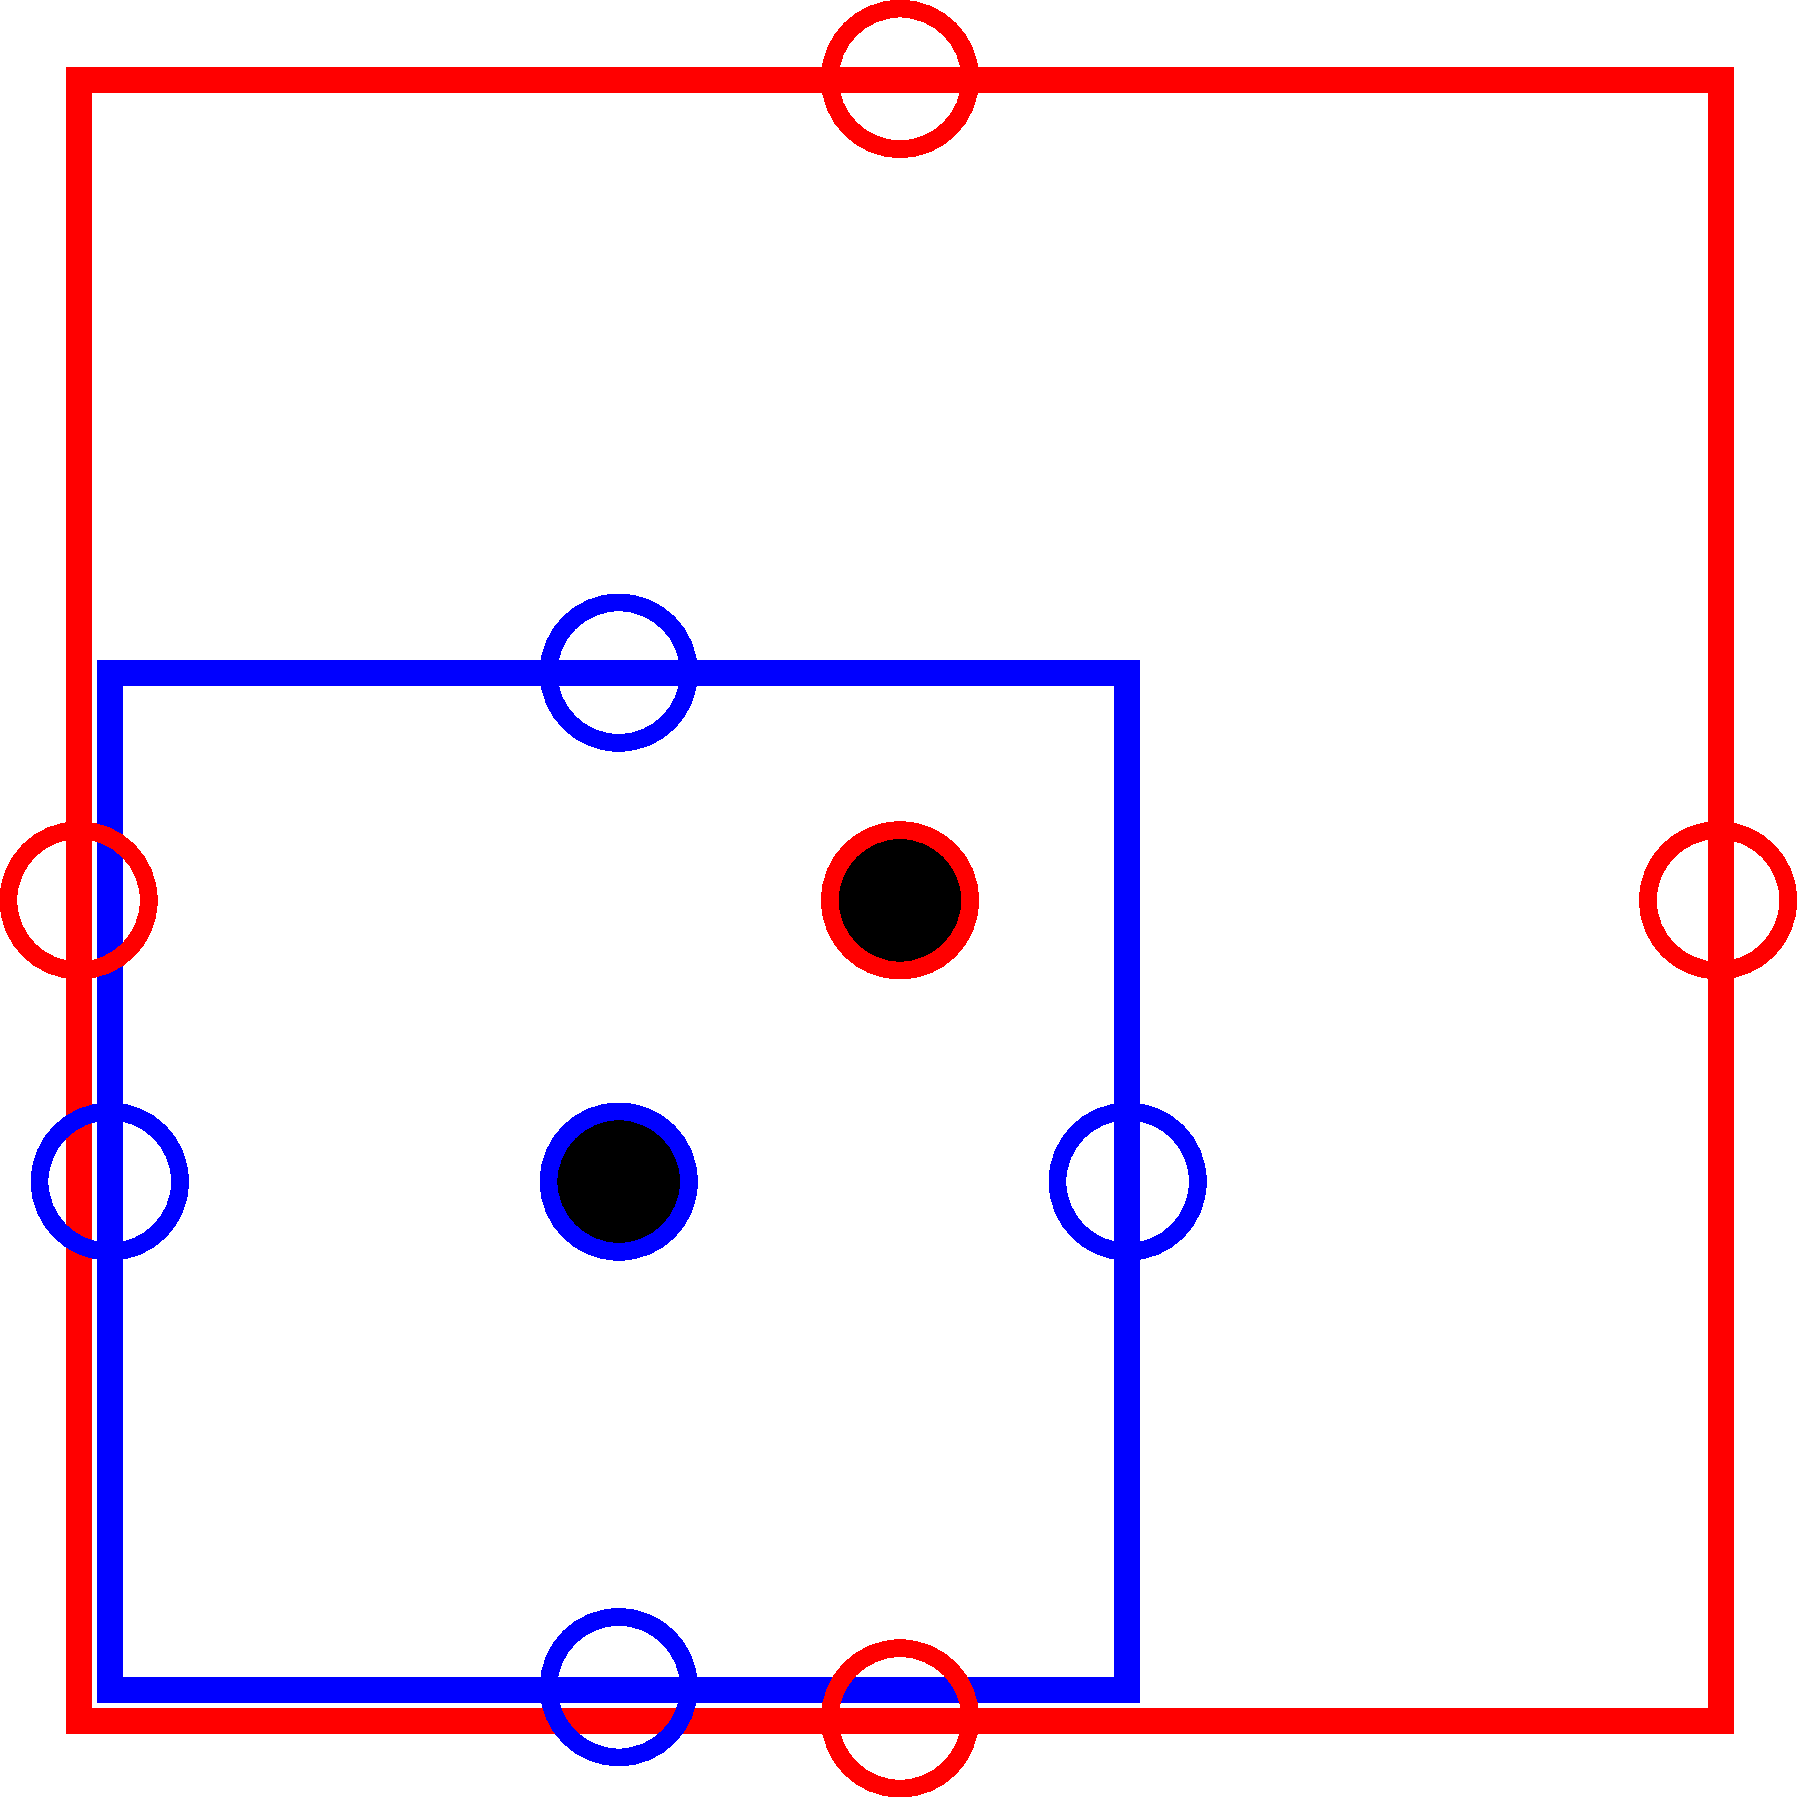
\includegraphics[width=0.6\textwidth]{drawings/audtestsetup}
    \caption{The setup for Room 1 and Room 2 (illustration of \Cref{fig:audtest}). Room 1 is marked as the inner (blue) square and is $5 \times 5$ meters. Room 2 is marked as the outer (red) square and is $8 \times 8$ meters. The rings shows the position of the beacons. The filled circles shows where the the phone is placed to obtain the position (only for the non-moving tests).}
    \label{fig:audtestsetup}
\end{figure}

\FloatBarrier
\subsection{Room 2}

\subsection{Room 3}

\subsection{Room 4}

\subsection{Conclusion}


We setup a [SIZE OF ROOM] room, with [NUMBER OF BEACONS]. 
The room is illustrated by \Cref{fig:precisiontest}. 
In \Cref{fig:precisiontest} you can also see small spots. 
These spots is the known locations where we are going to perform the precision tests. 
We randomly walk between these spots [NUMBER OF TIMES] and find the mean error rate.
\begin{figure}[!htb]
    \centering
    \todo[author=Thalley]{Insert figure}
    \caption{Illustration of room used for indoor location precision test}
    \label{fig:precisiontest}
\end{figure}

The mean error rate that we found is [RESULT]. 

\subsection{Precision of Indoor Location Conclusion}
From the results, we can conclude that... \todo[author=Thalley]{Write conclusion of precision test based on results}


\section{Pointing}
\label{sec:evaluation:pointing}

A qualitative test of pointing with the device, 
as described in \Cref{sec:detecting-points}, 
was performed. 
We were interested in determining if we are able to determine, 
when users point with the device, 
and when it lies on the table.

In order to perform the test, 
we isolated the point detector in a small application, 
that would show a white screen when no point was detected. 
When a point was detected, 
the application would show stop detecting points, 
and show a green screen for five seconds, 
and then start detecting points again.
This gave us a visual confirmation that a point was detected.

The test was performed by walking around a room, 
stopping up and pointing at an object. 
This was performed multiple times, 
and in all cases the screen successfully turned green.

Furthermore we put the phone down on various tables inside the room. 
The screen remained white and thus not points were detected.

During our tests we did find the following two issues:
\begin{itemize}
\item Detecting a point felt slow. The time that passes from the user points with the device to the point is detected, is too long. This could possibly be fixed by reducing the length of the sampling period, but this may have an impact on the accuracy of the detector, \ie it may detect points when the user did not intend to point.
\item When the phone lied still on a table with small vibrations, it would detect a point. For example, typing on a laptop placed on a table, caused the table to make small vibrations. In this case, the detector may recognize a point. This could possibly be fixed by increasing the acceleration threshold for tables. However, this may negatively impact the accuracy of the detector when the user points.
\end{itemize}

%%% Local Variables:
%%% mode: latex
%%% TeX-master: "../../master"
%%% End:

\section{Server and HomePort}\label{sec:servereval}
This section briefly describes the evaluation of the implemented server and HomePort. 

The server has not been tested in detail, 
as the number of the requests send to and from the server is small,
and the complexity of the requests are simple. 
We have experienced no problems with the server during development,
or through testing the application. 

HomePort on the other hand have showed problems. 
The implementation of HomePort that we use, 
is the so-called OldHomePort\footnote{\url{https://github.com/home-port/HomePort/tree/OldHomePort}}. 
We used this version as it was the only one with a phidget adapter implemented. 
Through testing we have found that this version of HomePort crash a lot when receiving requests. 
Sometimes it will even disconnect the phidget interface kit, 
and thus all the devices, at seemingly random points of time. 
We have not worked on determining the errors of OldHomePort, 
nor have we tried to debug it. 
This is primarily because it is a third-party component of our system, 
and have only been used to properly test the communication between the devices and the phone. 
\section{System Correctness}
\label{sec:evaluation:system-correctness}

In order to determine the system correctness, 
given the inaccuracy of the indoor positioning described in \Cref{sec:estimoteprecision}, 
we created a simulation of the system.

The purpose of the simulation is to calculate how often the user \emph{actually} points at the intended device, 
given some inaccuracy of the indoor positioning.

The system is based on multiple \textit{setups}. 
Each setup consists of the following parameters:
\begin{itemize}
\item \texttt{roomSize}: The size of some room.
\item \texttt{position}: A position of the user in the room.
\item \texttt{devices}: The devices available in the room.
\item \texttt{focusedDevice}: The device the user must point at.
\item \texttt{offset}: An offset applied to the users position.
\end{itemize}

For each setup, the simulation calculates the orientation the user must have in order to point at \texttt{focusedDevice}. 
The simulation then performs \num{100} tests for each setup. 
For each of those tests, 
the user's position is offsetted both horizontally and vertically, 
by a total amount of \texttt{offset}. 
The horizontal offset, \ie the offset for $x$, 
is chosen as a random number between $-\var{offset}$ and $\var{offset}$. 
The vertical offset, \ie the offset for $y$, 
is then calculated as $y = \sqrt{\var{offset}^2 - x^2}$. 
We then ensure that $x \geq 0 \wedge x \leq \var{roomSize.width} \wedge y \geq 0 \wedge y \leq \var{roomSize.height}$.

One iteration of the test consists of multiple setups, 
with different values for \texttt{position} and \texttt{focusedDevice}. 
We had three setups for each device in the system. 
Six devices were included resulting in a total of 18 setups.

For each of the \num{18} setups we performed \num{100} tests with different offsets of the user. 
In each of the \num{100} tests, 
we found the set of devices the user points at given his position, 
his orientation and the set of six devices. 
If the \texttt{focusedDevice} is still in the set of devices the user points at, 
\ie the user points at the intended device,
the test is considered to be accepted. 

The result of performing the \num{1800} tests, 
is a percentage of how often the \texttt{focusedDevice} was in the set of visible devices. 
For example, a test result of \perc{24} indicates that \perc{24} of the time, 
the user still pointed at the desired device, 
even though his location was offset, as it would be if we got the position from the Estimote Indoor SDK.

Since there are random numbers in the system, 
we may get slightly different results when performing a test with the exact same input values. 
Therefore we perform the \num{1800} tests \num{10} times each, 
and take the average correctness rate.

This was performed seven times with different offsets in order to see the influence of \texttt{offset},
\ie the influence of the inaccuracy of Estimote.

To sum up:
\begin{enumerate}
\item We tested a number of setups. In our case this is \num{18}, three for each of the six devices in the system.
\item \num{100} tests for each of the setups. Each test randomly offsets the user position horizontally and vertically resulting in a total offset of \texttt{offset}.
\item The set of \num{18} setups is then tested \num{10} times in order to calculate an average accuracy. This results in \num{18000} small tests where the users position is offsetted.
\item This is then done seven times with different values of \texttt{offset}.
\end{enumerate}

\subsection{Configuration}

\Cref{tbl:evaluation:system-correctness:devices} shows the six devices used in the simulation of the system.

\begin{table}[!hbt]
\centering
\caption{Devices used in the simulation.}
\label{tbl:evaluation:system-correctness:devices}
\begin{tabular}{c|c}
	\textbf{ID} & \textbf{Coordinate} \\ \hline
	     1      &    $(6.5, 3.4)$     \\
	     2      &    $(3.5 , 3.4)$    \\
	     3      &    $(4.0 , 1.8)$    \\
	     4      &    $(2.5 , 1.8)$    \\
	     5      &    $(0.5 , 0.5)$    \\
	     6      &    $(2.5 , 3.2)$
\end{tabular}
\end{table}

\Cref{lst:evaluation:system-correctness:setups} shows the \num{18} setups tested. 
The set of setups was tested with the offsets shown in \Cref{lst:evaluation:system-correctness:results}, 
along with the achieved accuracy, 
when applying the offset to the users position.

The size of the room used in the setups, 
matches a real world living room in a \SI{80}{\square\meter} apartment. 
Six devices are used, 
as we found it reasonable in a living room of that size.

The positions used are arbitrary, 
and less important when we calculate the orientation, 
based on the users position and the position of the focused device.

\begin{table}[!hbt]
\centering
\begin{tabular}{c|ccc}
	\textbf{ID} & \textbf{Position} & \textbf{Focused device ID} & \textbf{Room size in meter} \\ \hline
	     1      &   $(2.0 , 2.0)$   &             1              &      $6.9 \times 5.37$      \\
	     2      &   $(3.4 , 4.9)$   &             1              &      $6.9 \times 5.37$      \\
	     3      &   $(1.1 , 3.6)$   &             1              &      $6.9 \times 5.37$      \\
	     4      &   $(0.5 , 0.5)$   &             2              &      $6.9 \times 5.37$      \\
	     5      &   $(1.1 , 3.3)$   &             2              &      $6.9 \times 5.37$      \\
	     6      &   $(5.5 , 5.2)$   &             3              &      $6.9 \times 5.37$      \\
	     7      &   $(3.0 , 2.9)$   &             3              &      $6.9 \times 5.37$      \\
	     8      &   $(1.0 , 2.0)$   &             3              &      $6.9 \times 5.37$      \\
	     9      &   $(2.5 , 2.3)$   &             3              &      $6.9 \times 5.37$      \\
	    10      &   $(4.4 , 3.4)$   &             4              &      $6.9 \times 5.37$      \\
	    11      &   $(6.0 , 1.2)$   &             4              &      $6.9 \times 5.37$      \\
	    12      &   $(5.8 , 2.7)$   &             4              &      $6.9 \times 5.37$      \\
	    13      &   $(4.6 , 1.4)$   &             5              &      $6.9 \times 5.37$      \\
	    14      &   $(2.3 , 5.2)$   &             5              &      $6.9 \times 5.37$      \\
	    15      &   $(0.3 , 0.1)$   &             5              &      $6.9 \times 5.37$      \\
	    16      &   $(6.2 , 4.4)$   &             6              &      $6.9 \times 5.37$      \\
	    17      &   $(5.1 , 2.7)$   &             6              &      $6.9 \times 5.37$      \\
	    18      &   $(3.2 , 5.1)$   &             6              &      $6.9 \times 5.37$
\end{tabular}
\caption{Setups used in the simulation. Device IDs references table \ref{tbl:evaluation:system-correctness:devices}.}
\label{lst:evaluation:system-correctness:setups}
\end{table}

During all tests a visibility angle of \num{30} degrees was used, 
\ie \num{15} degrees on each side of the users orientation, 
as described in \Cref{sec:analysis:orientation}.

\Cref{fig:evaluation:system-correctness:simulation} illustrates the simulation. 
In this case the user desires to control Device 1 (the rightmost device). 
The figure shows three situations in the simulation. 
\Cref{fig:evaluation:system-correctness:simulation:initial} shows the initial situation, 
in which the user faces the device directly. 
This situation is not considered when calculating the resulting accuracy, 
as this situation always takes place when the orientation of the user is calculated. 
The \emph{accepted} situation is shown in \Cref{fig:evaluation:system-correctness:simulation:accepted}. 
Even though the user's location is offsetted, 
Device 1 is still in his line of sight. 
This is not the case in \Cref{fig:evaluation:system-correctness:simulation:failure}, 
where the offset causes Device 1 to no longer be in the user's line of sight.

Please note that the line of sight in \Cref{fig:evaluation:system-correctness:simulation} is for \emph{illustration purposes only}. 
In reality the line of sight is a triangle of \num{30} degrees, 
from the user pointing in the users orientation.

\begin{figure}[!htb]%
    \centering
    \subbottom[Initial position of the user. The user focuses directly on Device 1 (the rightmost device).]{\label{fig:evaluation:system-correctness:simulation:initial}
        \frame{\includegraphics[width=0.3\textwidth]{images/system-correctness-initial}}
    }
    \subbottom[Accepted position of the user. Even though the user's location is offsetted, Device 1 is still in his line of sight.]{\label{fig:evaluation:system-correctness:simulation:accepted}
        \frame{\includegraphics[width=0.3\textwidth]{images/system-correctness-accepted}}
    }
    \subbottom[Rejected position of the user. Due to the offset, Device 1 is no longer in the users line of sight.]{\label{fig:evaluation:system-correctness:simulation:failure}
        \frame{\includegraphics[width=0.3\textwidth]{images/system-correctness-failure}}
    }
    \caption{Illustrations of the simulation. Device 1 is the desired device to be focused.}
    \label{fig:evaluation:system-correctness:simulation}
\end{figure}

\subsection{Results}

\Cref{lst:evaluation:system-correctness:results} shows the results of the simulation. 
We tested the system with offsets from \SI{0}{\meter} to \SI{2.92}{\meter} with a \SI{0.5}{\meter} interval. 
We test up to \SI{2.92}{\meter}, 
as this is the average accuracy we measured when testing the precision of Estimote, 
as described in \Cref{sec:estimoteprecision}.

\begin{table}[!htb]
	\centering
	\begin{tabular}{rc}
		  \textbf{Offset} & \textbf{Percentage of correct points} \\ \hline
		   \SI{0}{\meter} &             \perc{100.00}             \\
		 \SI{0.5}{\meter} &             \perc{88.93}              \\
		   \SI{1}{\meter} &             \perc{56.67}              \\
		 \SI{1.5}{\meter} &             \perc{23.54}              \\
		   \SI{2}{\meter} &             \perc{12.56}              \\
		 \SI{2.5}{\meter} &              \perc{6.89}              \\
		\SI{2.92}{\meter} &              \perc{4.29}
	\end{tabular}
	\caption{Results of the seven tests performed. The ``Offset'' column shows the total offset applied to the users position, and the ``Accuracy'' column shows the number of tests, that resulted in the desired device being in the line of sight. The percentage has been rounded to two decimals.}
	\label{lst:evaluation:system-correctness:results}
\end{table}

\begin{figure}[!htb]
    \centering
    \begin{tikzpicture}
  \begin{axis}[
%      ybar,
%      bar width=2pt,
      xlabel = Offset in meters,
      ylabel = Accuracy in percent,
      xtick=data,
      width=0.95\textwidth,
      height = 6cm,
      yticklabel style={align=right,inner sep=0pt,xshift=-0.3em},
      enlargelimits = false,
      ymax = 100,
      grid=major,
      try min ticks=10]]
    \addplot table[x=offset, y=accuracy] {data/system-correctness/results.csv};   
  \end{axis}
\end{tikzpicture}
    \caption{Accuracy of the system for each of the offsets in table \ref{lst:evaluation:system-correctness:results}.}
    \label{fig:evaluation:system-correctness:results}
\end{figure}

Based on the results presented in \Cref{lst:evaluation:system-correctness:results} and illustrated by \Cref{fig:evaluation:system-correctness:results}, 
we can conclude that the system is \emph{not} sufficiently accurate. 
With a mean error of \SI{2.92}{\meter}, 
the system will only point at the desired device \perc{4.29} of the time. 
In order to achieve the desired accuracy of \perc{80} described in the requirements section (\Cref{sec:requirements-specification}), 
we must reduce the offset to less than \SI{\sim 0.6}{\meter}.

Inaccuracy in the orientation of the user, 
which may the result of an inaccurate magnetometer, 
was not simulated in this test. 
From use throughout the project, 
we generally found the magnetometer to be reliable within a few ($\sim 5$) degrees. 
Any inaccuracy in the measurements provided by the magnetometer, 
could be compensated by a wider visibility angle.

%%% Local Variables:
%%% mode: latex
%%% TeX-master: "../../master"
%%% End:

% \section{Overall System Correctness}\label{sec:systemcorrectness}
This test is designed to test the system as a whole. 
We want to test how many times the system:
\begin{enumerate}
    \item Sends the right action to the right device
    \item Sends the wrong action to the right device
    \item Sends the right action to the wrong device
    \item Sends the wrong action to the wrong device
\end{enumerate}
Thus this test is meant to total correctness of our system. 

We have the following setup, also illustrated in \Cref{fig:totalcorrectness}:
[SETUP: Which devices, where they are, where we stand, etc.]
\begin{figure}[!htb]
    \centering
    \todo[author=Thalley]{Insert figure}
    \caption{Illustration of our setup for the total correctness test}
    \label{fig:totalcorrectness}
\end{figure}

We send a total of [NUMBER OF GESTURES]. 
\Cref{table:correctnessresults} shows the results of this test.

\begin{table}
    \centering
    \begin{tabular}{l|cc}
                     & Right action & Wrong Action \\ \hline
        Right Device &      x       &     z        \\
        Wrong Device &      y       &     w        \\
    \end{tabular} 
    
    \todo[author=Thalley]{Insert results}
    \caption{Table showing the correctness of our system}
    \label{table:correctnessresults}
\end{table}

\subsection{Overall System Correctness Conclusion}
From the results, we can conclude that... \todo[author=Thalley]{Write conclusion of precision test based on results}
